%%%%%%%%%%%%%%%%%%%%%%%%%%%%%%%%%%%%%%%%%%%%%%%%%%%%%%
% A Beamer template for Ritsumeikan University       %
% Author: Ming-Hao Xu (Xu Minghao)                   %
% Date:   April 2022.                                %
% LPPL Licensed.                                     %
%%%%%%%%%%%%%%%%%%%%%%%%%%%%%%%%%%%%%%%%%%%%%%%%%%%%%%

\documentclass{beamer}
\usepackage{hyperref}

\usepackage[UTF8]{ctex}
\usepackage[T1]{fontenc}

% other packages
\usepackage{latexsym,amsmath,xcolor,multicol,booktabs,calligra}
\usepackage{graphicx,pstricks,listings,stackengine}
\usefonttheme[onlymath]{serif}

% dummy text; remove it when working on this template
\usepackage{lipsum}

\author{Ebola}
\title{计算几何2:旋转卡壳、三角形、圆}
\institute{
    Institute of Mathematics, \\
    Zhejiang University.
}
\date{Jan, 2024}
\usepackage{Ritsumeikan}

% defs
\def\cmd#1{\texttt{\color{red}\footnotesize $\backslash$#1}}
\def\env#1{\texttt{\color{blue}\footnotesize #1}}
\definecolor{deepblue}{rgb}{0,0,0.5}
\definecolor{deepred}{rgb}{0.6,0,0}
\definecolor{deepgreen}{rgb}{0,0.5,0}
\definecolor{halfgray}{gray}{0.55}

\lstset{
    basicstyle=\ttfamily\tiny,
    keywordstyle=\bfseries\color{deepblue},
    emphstyle=\ttfamily\color{deepred},    % Custom highlighting style
    stringstyle=\color{deepgreen},
    numbers=left,
    numberstyle=\small\color{halfgray},
    rulesepcolor=\color{red!20!green!20!blue!20},
    frame=shadowbox,
}


\begin{document}

\begin{frame}
    \titlepage
\end{frame}

\begin{frame}
    \tableofcontents[sectionstyle=show,subsectionstyle=show/shaded/hide,subsubsectionstyle=show/shaded/hide]
\end{frame}

\section{基础回顾}

\begin{frame}[fragile]{P2116 城墙}
有一次,一个贪婪的国王命令他的骑士在他的城堡外修建一堵围墙,要求围墙离城堡的最近距离不能少于 $L$。

城堡是一个 $n$ 边形,国王非常吝啬,不愿意多花建一米的围墙,多建的话他会杀掉负责修建的骑士。

请你帮助这个倒霉的骑士,帮他求出最少需要修建多长的围墙。
\end{frame}

\begin{frame}[fragile]{P2116 城墙}
答案是凸包周长 $+2\pi L$.

\begin{figure}[H]
    \centering
    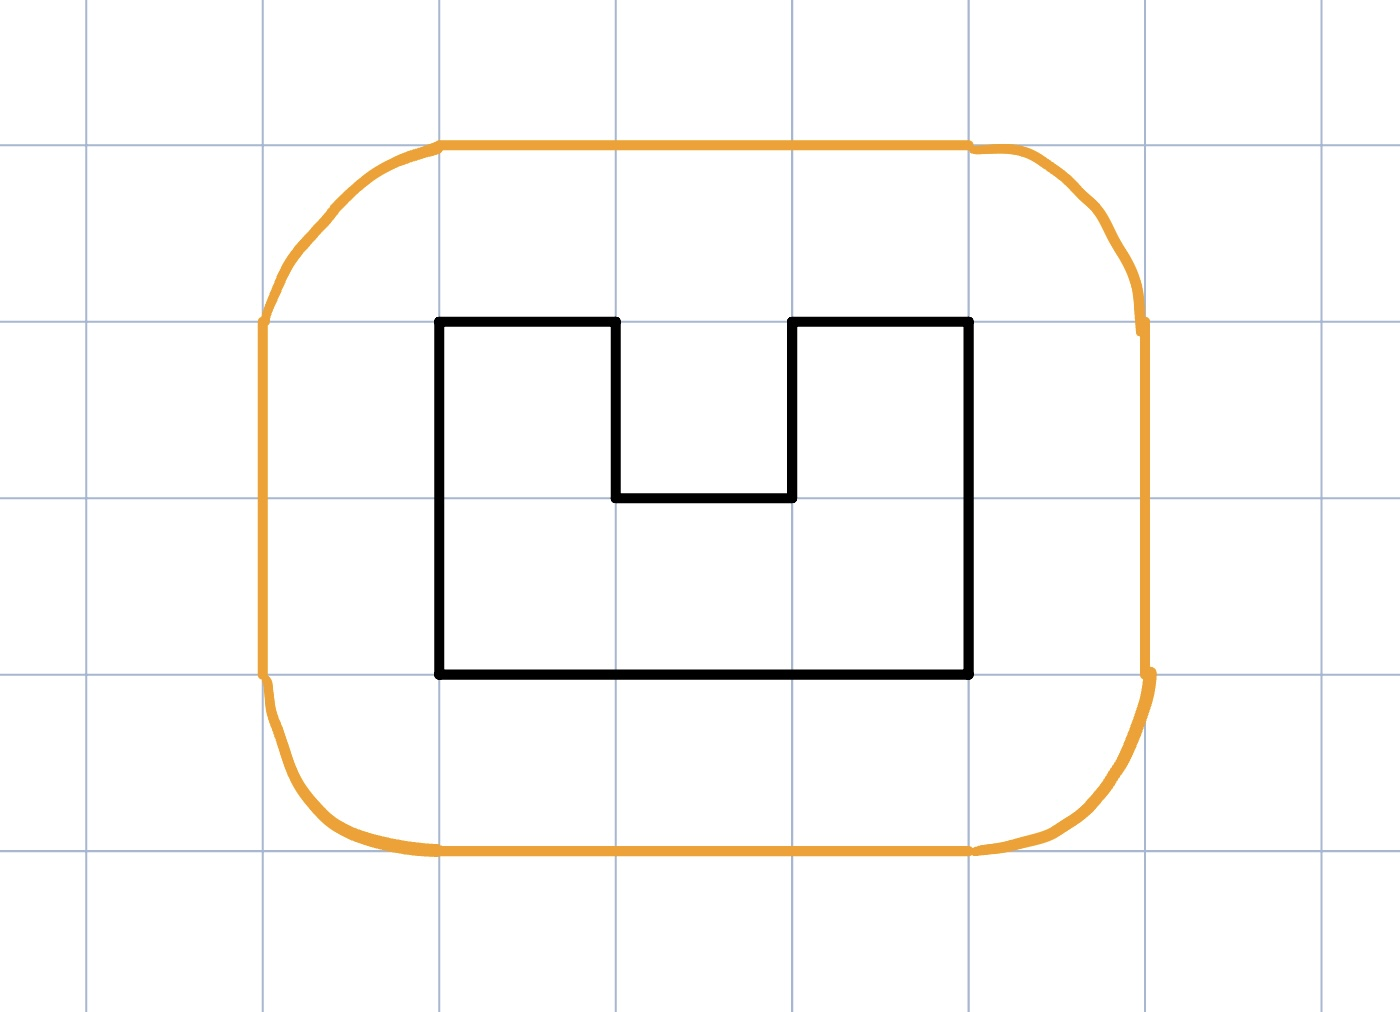
\includegraphics[width=0.7\textwidth]{pic/p2116.jpg}
\end{figure}
\end{frame}

\begin{frame}{[CERC2016] 凸轮廓线}
    一些几何图形整齐地在一个网格图上从左往右排成一列。它们占据了连续的一段横行,
    每个位置恰好一个几何图形。每个图形是以下的三种之一:

    \begin{enumerate}
        \item 一个恰好充满单个格子的正方形。
        \item 一个内切于单个格子的圆。
        \item 一个底边与格子重合的等边三角形。
    \end{enumerate}

    已知每个格子的边长都为 $1$,请求出这些几何图形的凸包的周长。

    \begin{figure}[H]
        \centering
        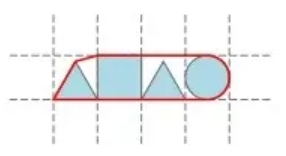
\includegraphics[width=0.5\textwidth]{pic/cerc2016.png}
    \end{figure}
\end{frame}

\begin{frame}{[CERC2016] 凸轮廓线}
    \small
    没什么好说的,
    非常非常复杂的分类讨论,
    极有可能漏掉一些情况!
\end{frame}

\begin{frame}{[ECNA2017] Craters(圆的凸包)}
    给定平面上 $n\;(\leq 200)$ 个圆的圆心坐标、半径,
    求能够围住所有圆的最短曲线的长度,精确到 $10^{-6}$。
\end{frame}

\begin{frame}{[ECNA2017] Craters(圆的凸包)}
    在每个圆上均匀地取 $T$ 个顶点,求这些顶点构成的凸包周长。

    \vspace{1em}
    $T$ 需要充分大。实测取 $2000$ 即可(比赛时尽量取大,反正 $5000$ 也不会炸)

    \vspace{1em}\pause
    一个有意思的结论:$T$ 每增大一倍,求得的周长的误差(即与精确周长之差的绝对值)
    缩小到原来的四分之一。(线性插值的二阶收敛性质)
\end{frame}

\begin{frame}[fragile]{向量的旋转}
    如果一个向量 $\overrightarrow{v}=(x,y)$,
    现在将它逆时针旋转 $90^\circ$,得到什么?

    \vspace{1em}\pause
    \begin{equation}
        \overrightarrow{v}^\perp=(-y,x).
    \end{equation}

\end{frame}

\begin{frame}[fragile]{向量的旋转}
    如果一个向量 $\overrightarrow{v}=(x,y)$,
    现在将它逆时针旋转 $\theta$,得到什么?

    \vspace{1em}\pause
    \begin{equation}
        \text{Rotate}(\overrightarrow{v},\theta)=(x\cos\theta-y\sin\theta,x\sin\theta+y\cos\theta).
    \end{equation}

\end{frame}

\begin{frame}[fragile]{点到直线的距离}
    \footnotesize
    给定 $P,A,B$ 三点坐标,求点 $P$ 到直线 $AB$ 的距离。(别用斜率)

    \vspace{1em}\pause
    \begin{figure}[H]
        \centering
        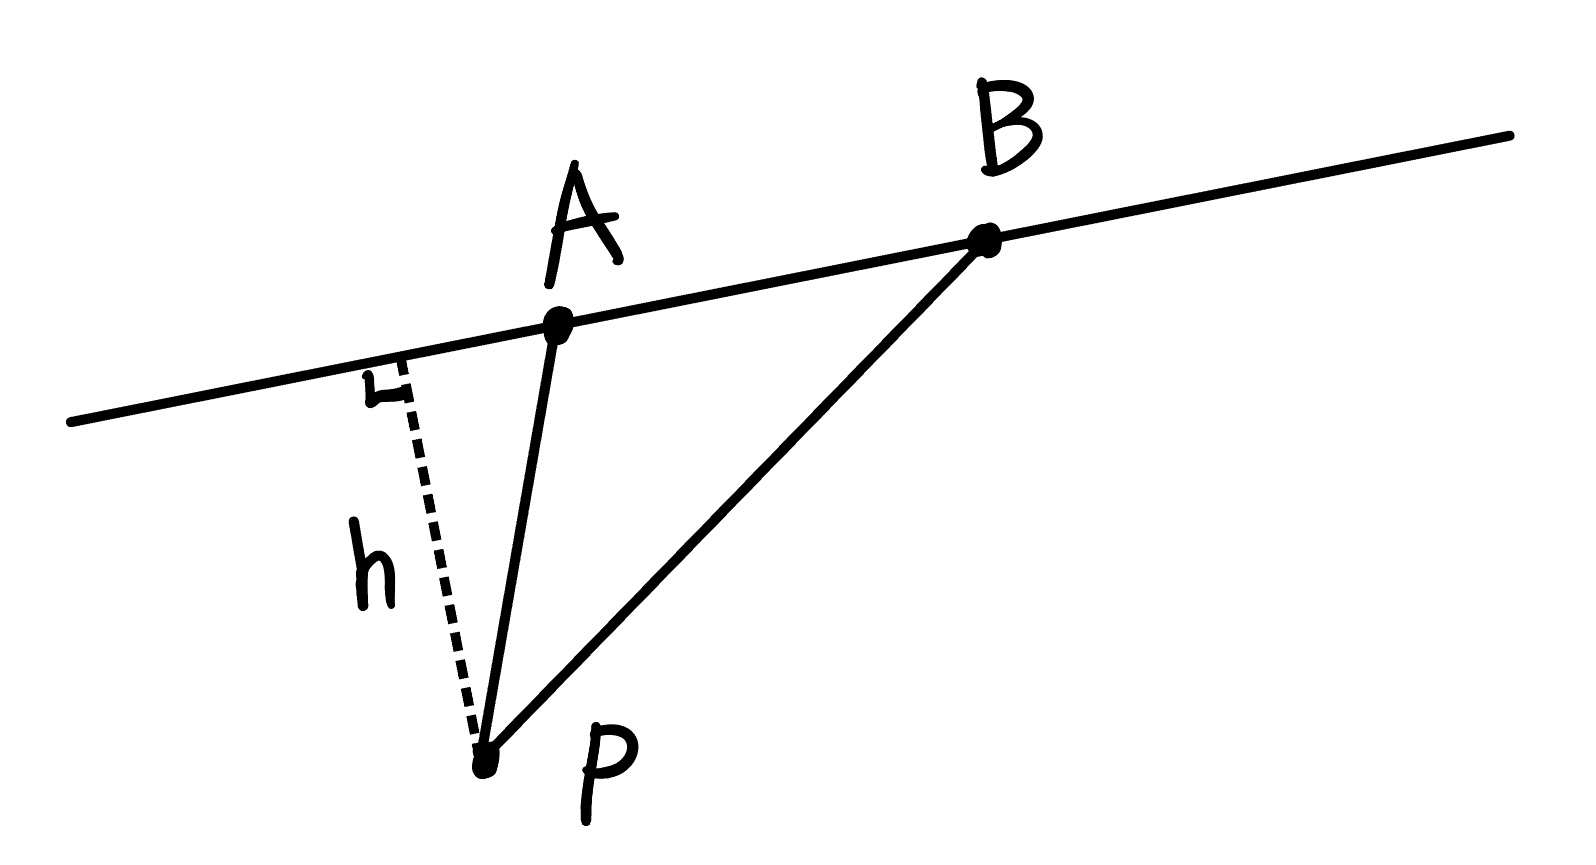
\includegraphics[width=0.5\textwidth]{pic/ptl.jpg}
    \end{figure}
    \begin{equation}
        h=\frac{S_{\Delta PAB}}{|AB|}=\frac{|\overrightarrow{PA}\times \overrightarrow{PB}|}{|AB|}.
    \end{equation}

    \vspace{1em}\pause
    \begin{lstlisting}[language=c++]
double DistanceToLine(Point P, Point A, Point B){
    return fabs(Cross(A-P, B-P)) / Length(A-B);
}
    \end{lstlisting}
\end{frame}

\section{旋转卡壳}

\begin{frame}{【模板】旋转卡壳}
    \small
    给定平面上 $n$ 个点,求凸包直径(直径是指最远的两个顶点的距离)。
\end{frame}

\begin{frame}{旋转卡壳}
    \small
    \begin{figure}[H]
        \centering
        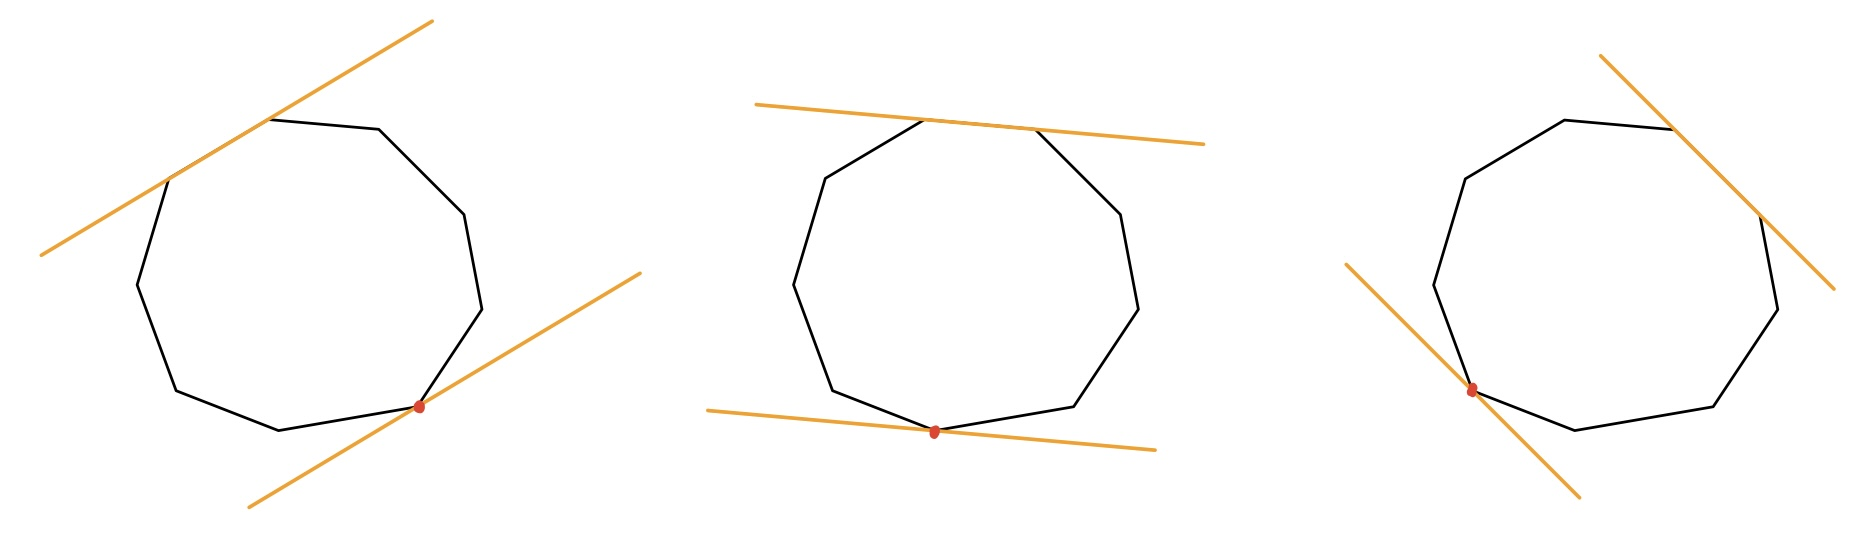
\includegraphics[width=\textwidth]{pic/rotation.jpg}
    \end{figure}
    如图所示,枚举上凸壳的边 $P_iP_{i+1}$,找到距离它最远的点。
    显然,当我们顺时针枚举边时,对面的点也只会顺时针方向前进,
    所以复杂度是 $O(n)$ 的。
\end{frame}

\begin{frame}[fragile]{旋转卡壳}
    \small
    \begin{lstlisting}[language=c++]
double RotatingCalipers(Point *ch, int n){
    if(n==2) return Length(ch[2] - ch[1]);
    int cur=0;
    double ans=0;
    ch[n+1] = ch[1];
    for(int i = 1; i <= n; i++){
        while(DistanceToLine(ch[cur], ch[i], ch[i+1]) 
           <= DistanceToLine(ch[cur%n+1], ch[i], ch[i+1])){
            cur = cur % n + 1;
        }
        ans=max(ans, max(Length(ch[i] - ch[cur]), 
                         Length(ch[i+1] - poly[cur])));
    }
    return ans;
}
    \end{lstlisting}
\end{frame}

\begin{frame}[fragile]{旋转卡壳}
    \footnotesize
    其实由于 $\Delta P_iP_{i+1}Q$ 的底边 $P_{i}P_{i+1}$ 是固定的,
    最大化 $Q$ 到直线 $l_{P_iP_{i+1}}$ 的距离就等价于最大化 $\Delta P_iP_{i+1}Q$
    的面积,因此不需要求点到直线的距离,直接调用叉乘即可,可以优化常数。
    \begin{lstlisting}[language=c++]
double RotatingCalipers(Point *ch, int n){
    if(n==2) return Length(ch[2] - ch[1]);
    int cur=0;
    double ans=0;
    ch[n+1] = ch[1];
    for(int i = 1; i <= n; i++){
        while(fabs(Cross(ch[i]-ch[cur], ch[i+1]-ch[cur])) 
           <= fabs(Cross(ch[i]-ch[cur%n+1], ch[i+1]-ch[cur%n+1]))){
            cur = cur % n + 1;
        }
        ans=max(ans, max(Length(ch[i] - ch[cur]), 
                         Length(ch[i+1] - poly[cur])));
    }
    return ans;
}
    \end{lstlisting}
\end{frame}

\begin{frame}[fragile]{旋转卡壳}
    \footnotesize
    还可以进一步优化常数,把两次叉乘简化成一次,\pause 只需要注意到:
    \begin{figure}[H]
        \centering
        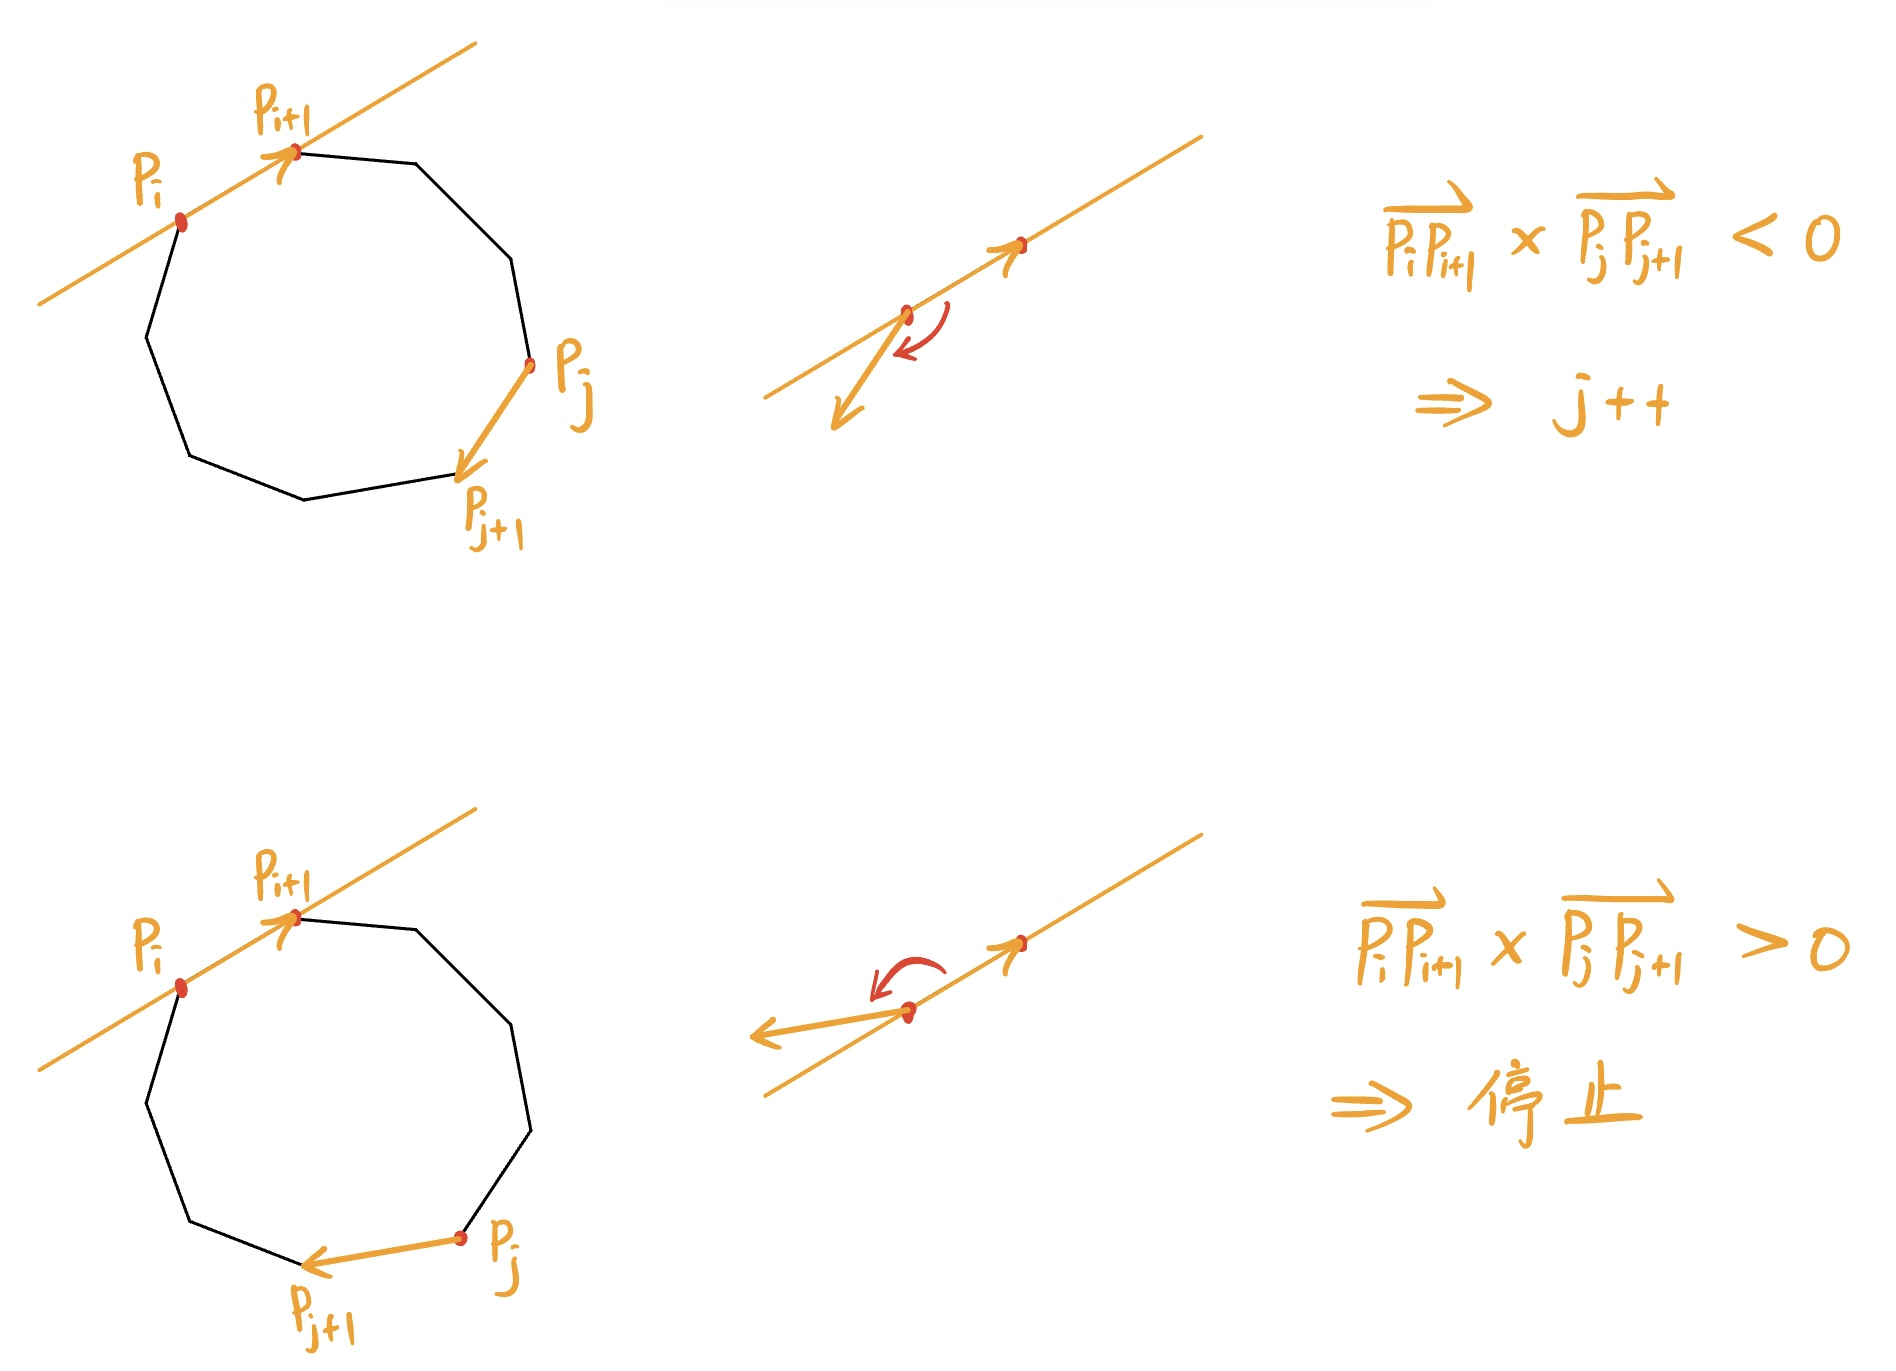
\includegraphics[width=0.7\textwidth]{pic/rotation_opt.jpg}
    \end{figure}
    \pause
    \begin{lstlisting}[language=c++]
while( Cross(ch[i+1]-ch[i], ch[cur%n+1]-ch[cur]) < 0 )
    \end{lstlisting}
\end{frame}

\begin{frame}{[HNOI2007] 最小矩形覆盖}
    \small
    给定一些点的坐标,求能够覆盖所有点的最小面积的矩形,
    输出所求矩形的面积和四个顶点坐标。
\end{frame}

\begin{frame}{[HNOI2007] 最小矩形覆盖}
    \footnotesize
    覆盖所有点等价于覆盖凸包的所有顶点,所以肯定先求凸包。

    \vspace{1em}\pause
    接下来都会想到旋转卡壳,像这样:
    \begin{figure}[H]
        \centering
        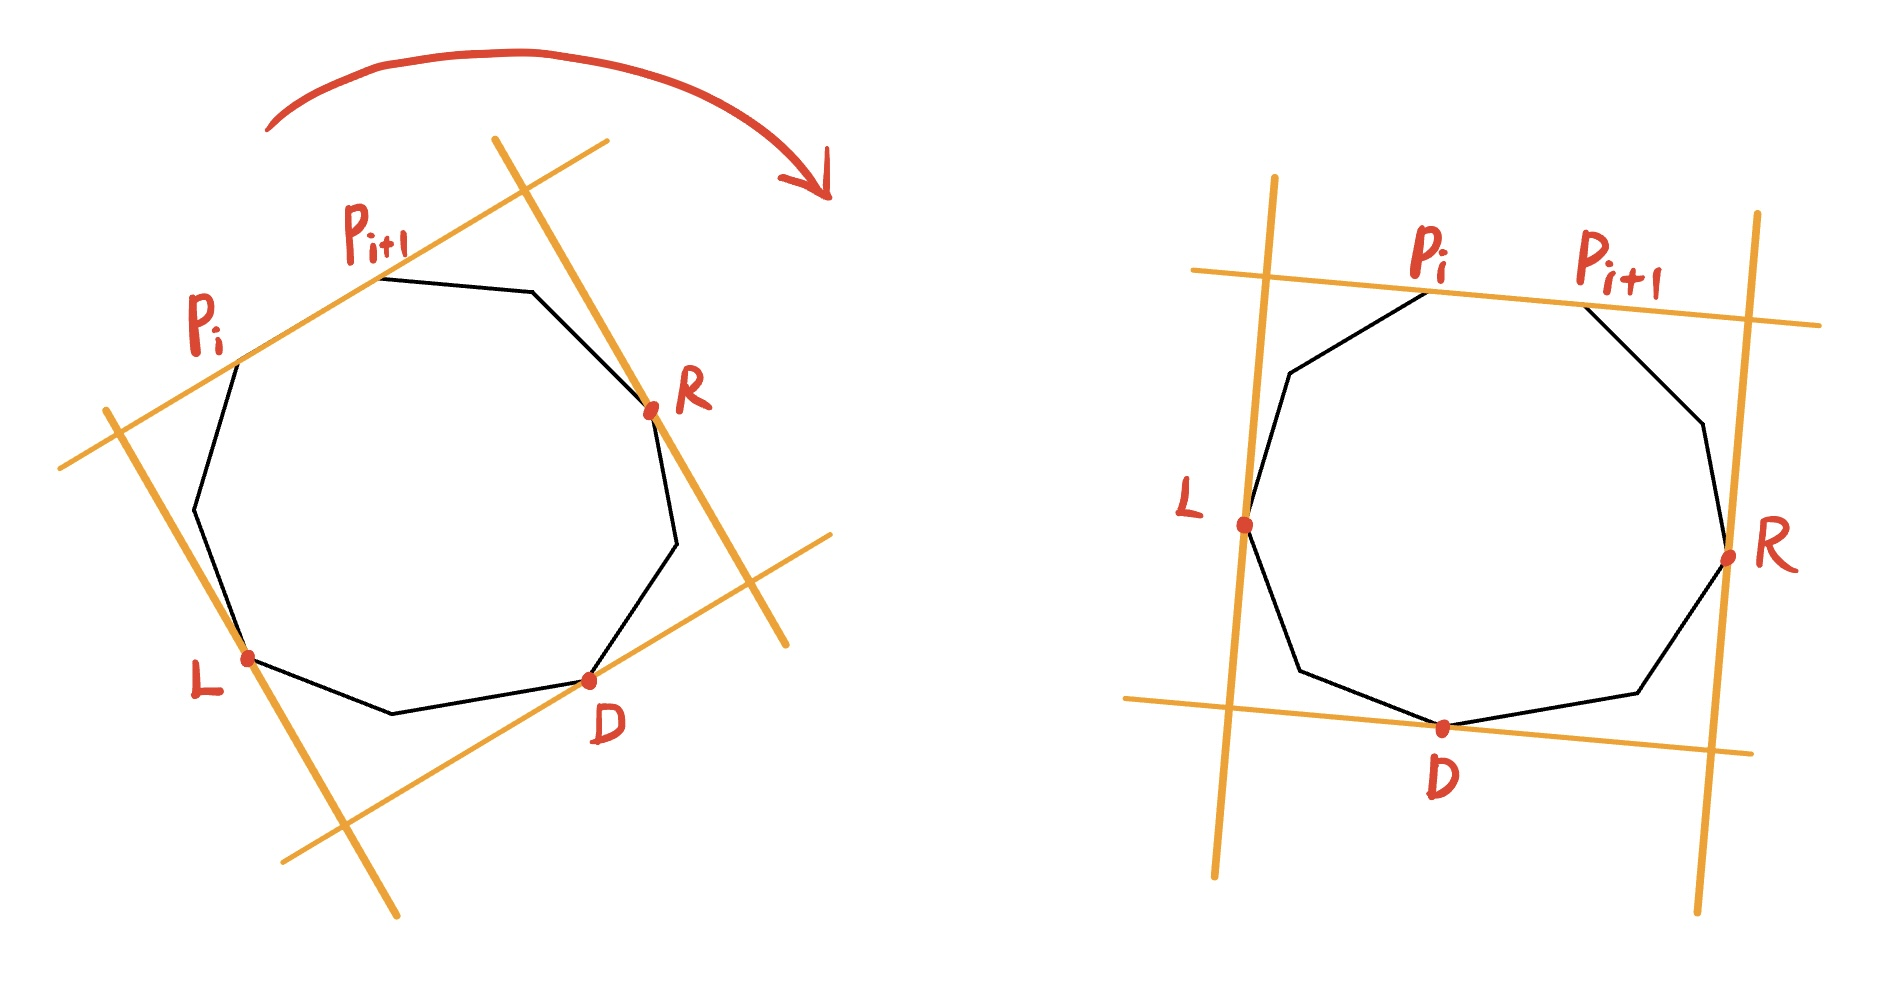
\includegraphics[width=0.8\textwidth]{pic/hnoi2007.jpg}
    \end{figure}
    然后按顺序枚举边 $P_{i}P_{i+1}$,并维护 $L,R,D$ 三个点。
    但是有一个问题。

    \vspace{1em}\pause
    为什么最小矩形一定有一条边和凸包的某条边重合?
    难道最小矩形不能每条边都只和凸包的一个顶点相切吗?
\end{frame}

\begin{frame}{[HNOI2007] 最小矩形覆盖}
    \footnotesize
    \textbf{结论:}最小矩形一定有一条边与凸包重合。

    \pause
    \textbf{证明:}若不然,即最小矩形的每条边都只和凸包的一个顶点相切。
    
    \begin{figure}[H]
        \centering
        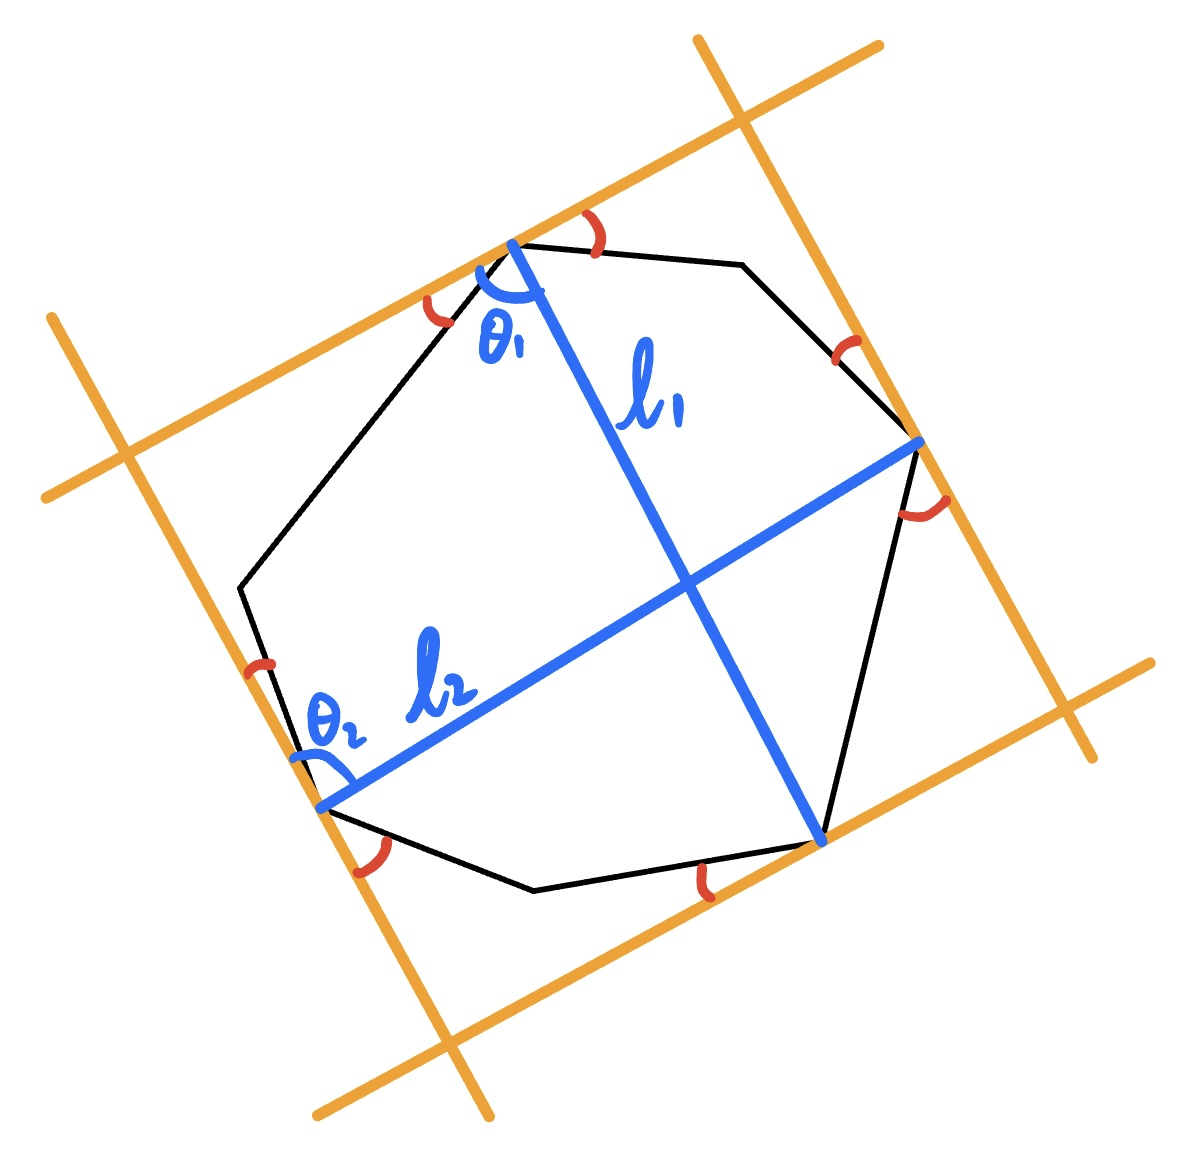
\includegraphics[width=0.25\textwidth]{pic/proof.jpg}
    \end{figure}

    \pause 此时面积是:$S=l_1\sin \theta_1\cdot l_2\sin \theta_2$.

    \pause 将矩形某条边
    旋转很小很小的 $\theta$ 角度
    (使标红的那些角仍然大于 $0$),
    另外三条边卡上去,新矩形的面积为:
    \begin{align}
        S' &= l_1\sin(\theta_1+\theta)\cdot l_2\sin(\theta_2+\theta)\\
        &= -\frac{1}{2}l_1l_2 \left(\cos(\theta_1+\theta_2-2\theta)-\cos(\theta_1-\theta_2)\right).
    \end{align}

    \pause 按照假设,必须当 $\theta=0$ 时 $S'$ 取得最小值。
    也就是说当 $\theta=0$ 时 $\cos(\theta_1+\theta_2-2\theta)$ 取得最大值。
    \pause 根据 $\cos$ 的性质我们必须有 $\theta_1+\theta_2=2k\pi$,这显然是不可能的,证毕!
\end{frame}

\begin{frame}[fragile]{[HNOI2007] 最小矩形覆盖}
    \footnotesize
    现在我们已经证明了结论,可以放心地卡壳了。

    \begin{lstlisting}[language=c++]
double RotatingCalipers(Point *ch, int n){
    int D = 0, L = -1, R = -1;
    double ans = 0;
    ch[n+1] = ch[1];
    for(int i = 1; i <= n; i++){
        while(DistanceToLine(ch[D], ch[i], ch[i+1]) 
            <= DistanceToLine(ch[D%n+1], ch[i], ch[i+1])){
            D = D % n + 1;
        }
        if(L==-1) L = i + 2;
        if(R==-1) R = D % n + 1;
        Point D2 = D + Rotate(ch[i+1]-ch[i], pi/2);
        while(DistanceToLine(ch[R], ch[D], D2) 
            <= DistanceToLine(ch[R%n+1], ch[D], D2)){
            R = R % n + 1;
        }
        while(...) L = L % n + 1;  // 自己写
        ans = max(ans, ...);       // 自己写
    }
    return ans;
}
    \end{lstlisting}
\end{frame}

\begin{frame}{[SCOI2007] 最大土地面积}
    \small
    给定一些点的坐标,选其中四个点,使它们构成的四边形面积最大。
    
    \vspace{1em}
    不超过 $2000$ 个点。(其实 $10^5$ 也能做)
\end{frame}

\begin{frame}[fragile]{[SCOI2007] 最大土地面积}
    \small
    旋转卡壳枚举对角线 $P_uP_v$,然后维护 $a,b$ 分别为
    $l_{P_uP_v}$ 两侧距离该直线最远的点。下面是确定 $u,v$ 后维护 $a,b$ 的代码。

    \begin{lstlisting}[language=c++]
void chkmx(int u, int v, int &a, int &b) {
    while ((a + 1) % n != v && 
           distance_to_line(p[a+1], p[u], p[v]) > 
           distance_to_line(p[a], p[u], p[v]))
        a = (a + 1) % n;
    while ((b + 1) % n != u && 
           distance_to_line(p[b+1], p[u], p[v]) > 
           distance_to_line(p[b], p[u], p[v]))
        b = (b + 1) % n;
    ans = max(ans,
            length(p[u] - p[v]) * 
            (distance_to_line(p[b], p[u], p[v]) 
            + distance_to_line(p[a], p[u], p[v])));
}
    \end{lstlisting}
\end{frame}

\begin{frame}{ [SDCPC2023] Computational Geometry}
    \footnotesize
    给定一个有 $n$ 个顶点的凸多边形 $P$,
    您需要选择 $P$ 的三个顶点,
    按逆时针顺序记为 $a$,$b$ 和 $c$。
    要求在 $b$ 沿逆时针方向到 $c$ 之间恰有 $k$ 条边
    (也就是说,$a$ 不是这 $k$ 条边的端点)。

    考虑用线段 $ab$ 和 $ac$ 将 $P$ 割开。将由线段 $ab$,$ac$,
    以及 $b$ 和 $c$ 之间的 $k$ 条边围成的 $(k + 2)$ 边形记作 $Q$。
    
    求 $Q$ 可能的最大面积。
    
    注意,$ab$ 和 $ac$ 可以与 $P$ 的边重合。

    \begin{figure}[H]
        \centering
        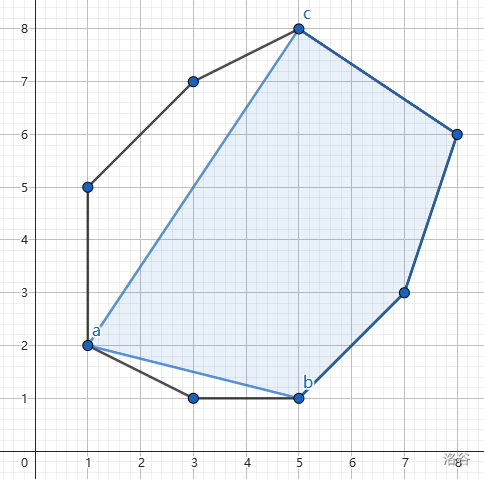
\includegraphics[width=0.5\textwidth]{pic/sdcpc2023sample.png}
    \end{figure}
\end{frame}

\begin{frame}{ [SDCPC2023] Computational Geometry}
    \small
    枚举 $b$,然后 $c$ 就确定了,接下来要让 $a$ 离 $l_{bc}$ 的距离最远,
    其实也就是旋转卡壳。
\end{frame}

\section{圆}

\begin{frame}{圆与直线的交点}
    \footnotesize
    给定直线上两个点 $A,B$ 的坐标、圆心 $P$ 的坐标、圆的半径 $r$,
    求直线 $l_{AB}$ 与圆的交点。

    \vspace{1em}\pause
    \begin{figure}[H]
        \centering
        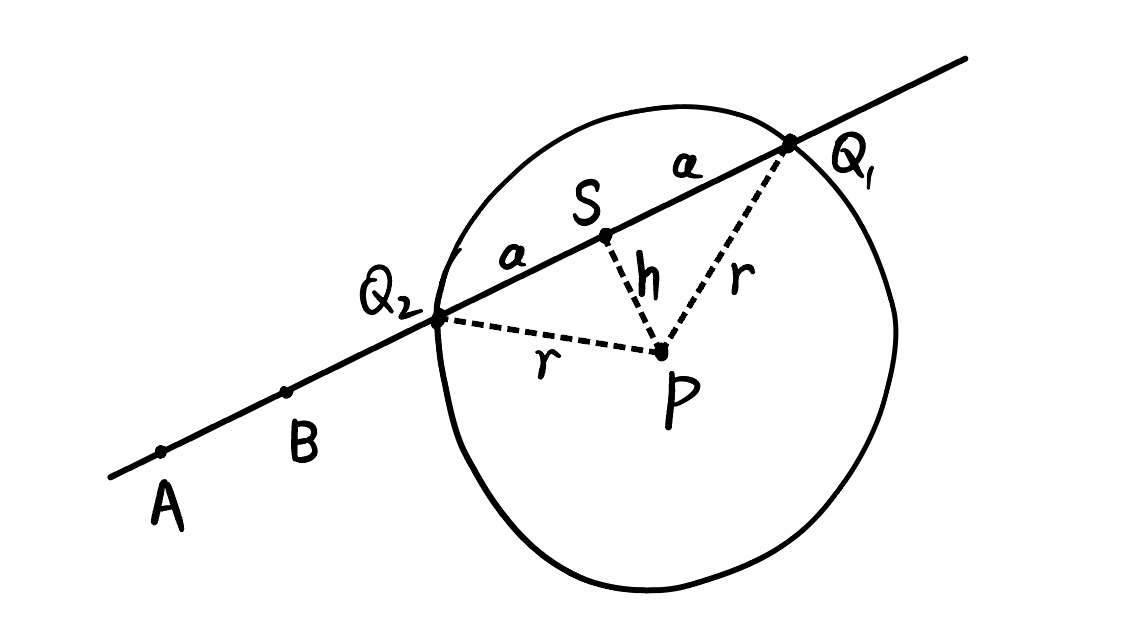
\includegraphics[width=0.4\textwidth]{pic/lineIcircle.jpg}
    \end{figure}
    先求出 $P$ 到 $l_{AB}$ 的距离 $h$,然后计算 $a=\sqrt{r^2-h^2}$,然后求出:
    \begin{align}
        S &= P+h \frac{\overrightarrow{AB}^\perp}{|AB|}\\
        Q_1 &= S + a \frac{\overrightarrow{AB}}{|AB|}\\
        Q_2 &= S - a \frac{\overrightarrow{AB}}{|AB|}
    \end{align}
\end{frame}

\begin{frame}{[BZOJ2178] 圆的面积并}
    给定 $n\;(n\leq 1000)$ 个圆,求它们覆盖区域的面积。
\end{frame}

\begin{frame}{[BZOJ2178] 圆的面积并}
    \footnotesize
    基本思路是辛普森积分求 $\int_L^R f(t)\; dt$,
    其中 $f(t)$ 表示直线 $x=t$ 与覆盖区域相交部分的长度。
    
    \vspace{1em}\pause
    对于一条直线 $x=t$,我们可以枚举所有圆,
    求出与该直线的所有交点,并从小到大排序,然后依次枚举;
    每碰到一个下交点,就加1,碰到上交点就减1;
    非零部分的总长度就是相交部分的长度。

    \begin{figure}[H]
        \centering
        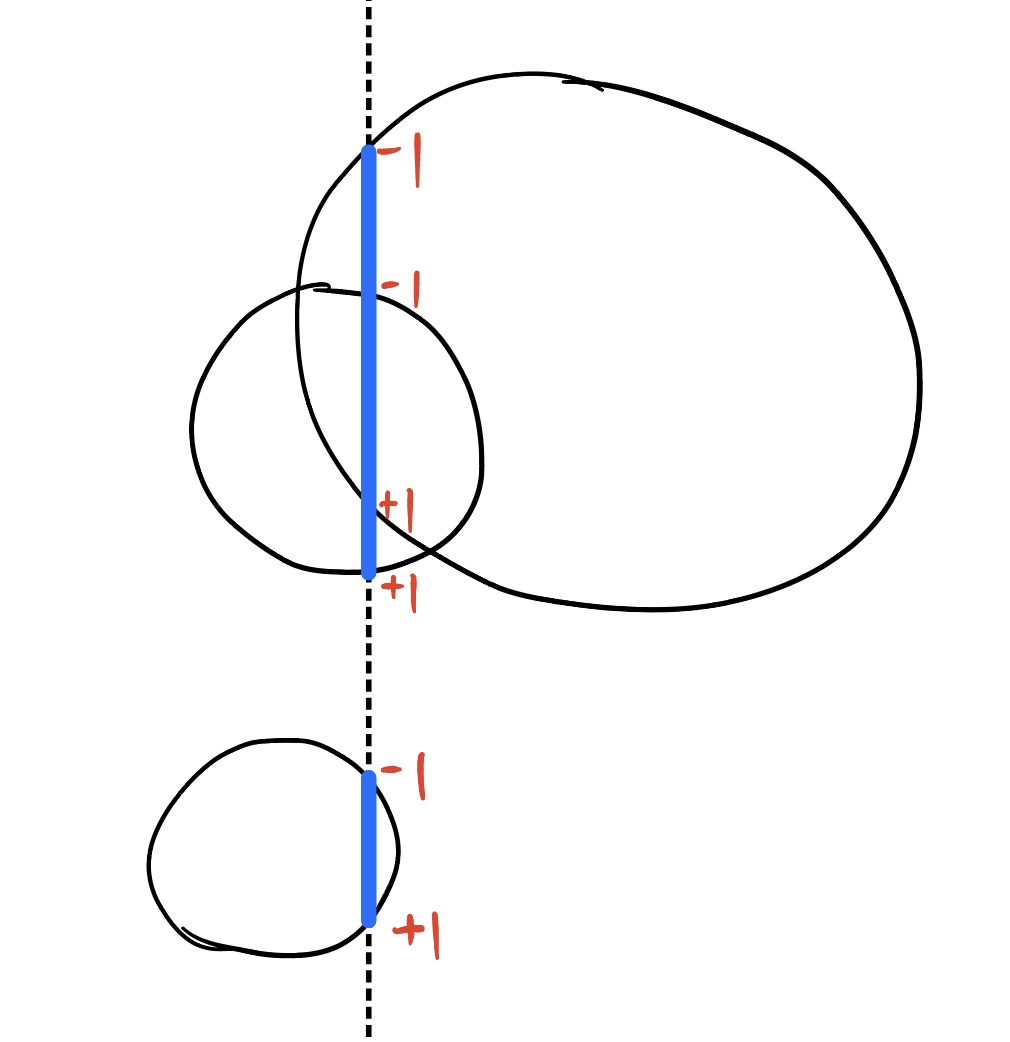
\includegraphics[width=0.4\textwidth]{pic/circleinsec.jpg}
    \end{figure}
\end{frame}

\begin{frame}{圆交}
    \small
    给定两个圆的圆心坐标 $P_1,P_2$,以及它们的半径 $r_1,r_2$,
    判断它们是否有交点(或切点),如果有,求之。
\end{frame}

\begin{frame}{正余弦定理}
    \small
    在求圆交之前,我们先来看两个三角形里的基本定理。

    \vspace{1em}\pause
    \begin{figure}[H]
        \centering
        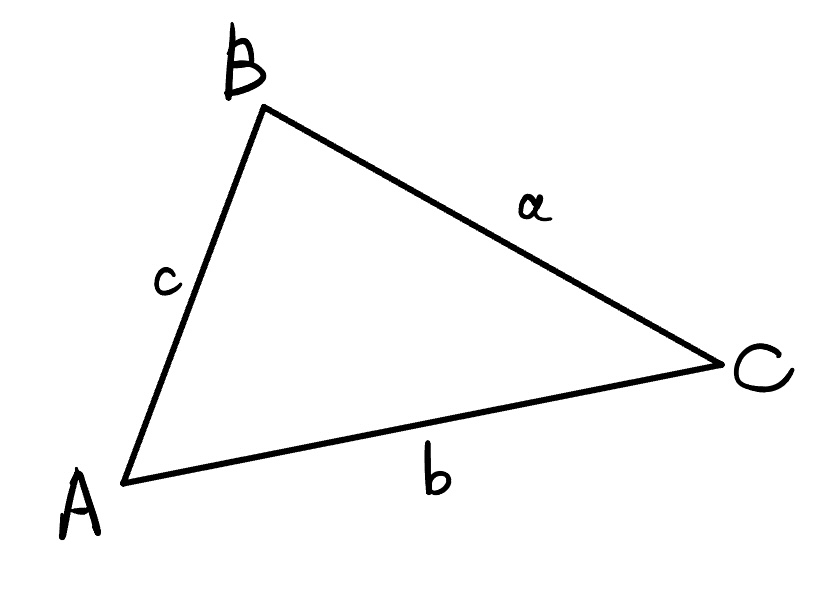
\includegraphics[width=0.4\textwidth]{pic/triangle.jpg}
    \end{figure}
    正弦定理:
    \begin{equation}
        \frac{\sin A}{a}=\frac{\sin B}{b}=\frac{\sin C}{c}.
    \end{equation}
    余弦定理:
    \begin{equation}
        \cos A=\frac{b^2+c^2-a^2}{2bc},\quad
        \cos B=\frac{a^2+c^2-b^2}{2ac},\quad
        \cos C=\frac{a^2+b^2-c^2}{2ab}. 
    \end{equation}
\end{frame}

\begin{frame}{圆交}
    \small
    \begin{figure}[H]
        \centering
        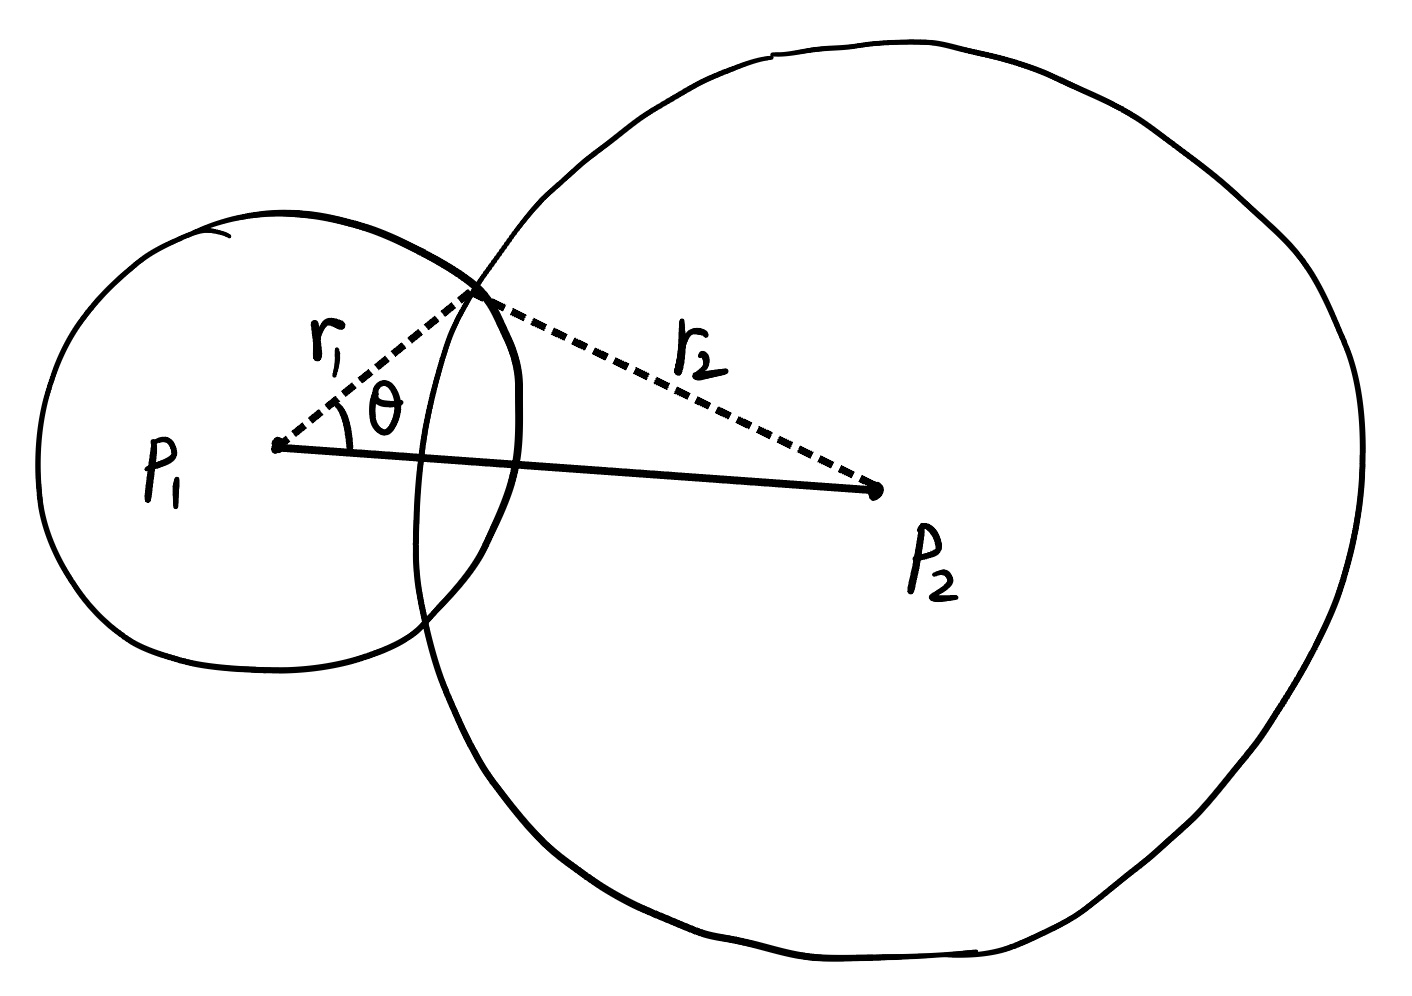
\includegraphics[width=0.5\textwidth]{pic/twocircle.jpg}
    \end{figure}
    先用余弦定理求出 $\theta$,\pause 然后求出第一个交点:
    \begin{equation}
        P_1+r_1\frac{\text{Rotate}(\overrightarrow{P_1P_2},\theta)}{|P_1P_2|}.
    \end{equation}
    第二个交点类似。
\end{frame}

\begin{frame}{[UVA10969] Sweet Dream}
    \small
    依次输入 $n$ 个圆的圆心坐标、半径,后输入的圆堆叠在先输入的圆上面,
    问最后可见部分的弧长总和。$T$ 组数据。($T,n\leq 100$)

    \begin{figure}[H]
        \centering
        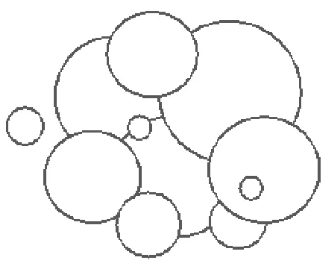
\includegraphics[width=0.5\textwidth]{pic/sweetdream.png}
    \end{figure}
\end{frame}

\begin{frame}{[UVA10969] Sweet Dream}
    \small
    对于第 $i$ 个圆,求出它和其它所有圆的交点,并将这些交点
    按逆时针排序。

    \vspace{1em}\pause
    这些交点将圆分成若干个圆弧,每个圆弧要么整个露出来,要么整个被挡掉。
    所以只要判断每个圆弧的中点是否位于某个圆 $j\;(>i)$ 内部即可。
    最后将露出来的圆弧长度累加。
\end{frame}

\begin{frame}{过定点作圆的切线}
    \small
    过圆外一点作圆的切线,求两个切点。
    \begin{figure}[H]
        \centering
        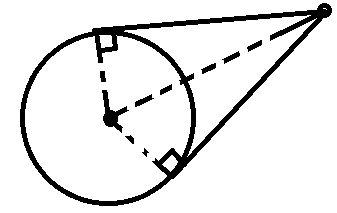
\includegraphics[width=0.5\textwidth]{pic/tangent.png}
    \end{figure}
\end{frame}

\begin{frame}[fragile]{过定点作圆的切线}
    \small
    直接用反正弦函数计算夹角,再由勾股定理计算切线段长度即可。
    \begin{lstlisting}[language=c++]
void circleTangent(Point P, double r, Point Q, Point &A, Point &B) {
    Vector v = Q - P;
    double c = Length(v);
    double b = sqrt(c*c - r*r);
    double theta = asin(r/c);
    A = Rotate(v, theta) / c * b;
    B = Rotate(v, -theta) / c * b;
}
    \end{lstlisting}
\end{frame}

\begin{frame}{求两圆的公切线}
    \small
    给定两个圆,求外公切线(上)和内公切线(下)。
    \begin{figure}[H]
        \centering
        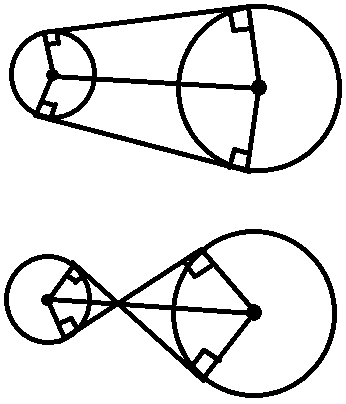
\includegraphics[width=0.5\textwidth]{pic/tangentTwoCircle.png}
    \end{figure}
\end{frame}

\begin{frame}{求两圆的公切线}
    \small
    注意,需要对圆的位置分类讨论切线是否存在。
    这里我们假设内外切线都存在,且都有两条,作辅助线:
    \begin{figure}[H]
        \centering
        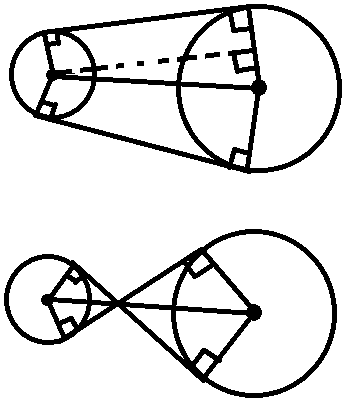
\includegraphics[width=0.5\textwidth]{pic/tangentTwoCircleFZ.png}
    \end{figure}

    算出需要的边长、角度即可。
\end{frame}

\begin{frame}{三点定圆}
    \small
    给出三角形的三个顶点 $(x_i,y_i)\;(i=1,2,3)$,求外接圆(用解析几何)。
\end{frame}

\begin{frame}{三点定圆}
    \small
    设圆心为 $(x,y)$,半径为 $r$,列方程:
    \begin{equation}
        (x-x_i)^2 + (y-y_i)^2 = r^2, \quad i=1,2,3.
    \end{equation}
    方程 $i\;(i=2,3)$ 减去方程 $1$,得到:
    \begin{equation}
        2(x_i-x_1)x + 2(y_i-y_1)y = x_i^2-x_1^2+y_i^2-y_1^2,\quad i=2,3.
    \end{equation}
    解线性方程即可得到 $x,y$,再代入方程 $1$ 求出 $r$.
\end{frame}

\begin{frame}
    \begin{center}
        {\Huge\calligra Thank You}
    \end{center}
\end{frame}

\end{document}